\section{Methodology}
\label{sec:methodology}

In this section we present the methodology of our experiment. We want to answer the following research questions:

\begin{enumerate}
	\item When in the history of projects is renaming located, and what is the typical amount of renaming?
	\item Is renaming able to skew significantly the values of change metrics?
\end{enumerate}

To answer these questions we conduct two successive experiments. In these experiments, we will use a dataset of five popular and mature open-source projects. As explained before, VCSs do not handle renaming out of the box, except Git. Therefore, the five projects we selected are managed by Git.

\subsection{First Experiment: Location and Amount}

Software projects usually undergo distinct phases in their life-cycle. Usually the development is started, then a version is released to the public and maintained, while a new version is being prepared, and so on. In our study we want to assess the amount of renaming in these phases. To that extent, we split a project history in various \emph{periods}. As described in \secref{changemetrics}, a period is a sequence of commits. Each period has a kind, as described in \figref{periods}. The \emph{init} kind is given to the period containing the commits from the beginning of the development to the first release. The \emph{dev} kind is given to periods where a release is being developed. The \emph{maint} kind is given to periods where a release is being maintained. In our project, we can distinguish dev and maint periods because the project we selected have separate branches for software maintenance and development. Our intuition concerning the amount of renaming it is the higher in the init period. Then it is from low to high in dev periods. Finally it is low in maint periods, because the maintenance phase is mostly dedicated to bug fixes.

\begin{figure}[t]
	\centering
	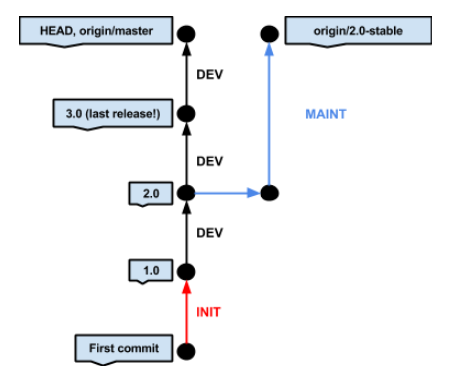
\includegraphics[width=1\linewidth,keepaspectratio]{data/figures/periods.png}
	\caption{Our period kinds, as follows. \emph{Init:} versions from the beginning (included) to the first release. \emph{Dev:} development versions between two successive releases. \emph{Maint:} maintenance versions for a specific release.}
	\label{fig:periods}
\end{figure}

To measure the location and amount of renaming in the projects, we manually extract the periods from the VCSs of our projects. For each period, we use the Git built-in algorithm to detect renamed files. Finally, for each period, we compute the following metrics:

\begin{itemize}
	\item \emph{Number of files ($\#F$):} number of files in the project at the last version of the period.
	\item \emph{Number of active files ($\#AF$):} number of files created, deleted, copied, modified or renamed during the period and present at the last version of the period.
	\item \emph{Percentage of active files ($\%AF$):} $\%AF = \frac{\#AF}{\#F}$.
	\item \emph{Number of renamed active files ($\#AF_{r}$):} number of active files that have been renamed.
	%\item \emph{Number of modification operations ($\#MO$):}  number of modifications (create, delete, copy, rename, modif) on files recorded in the location.
	%\item \emph{Number of rename operations ($\#RO$):} number of renames performed on the location.
	%\item \emph{Percentage of rename operations ($\%RO$):} \[ \%RO = \frac{\#RO}{\#MO}  \]
	\item \emph{Percentage of files renamed ($\%F_{R}$):} $\%F_{R} = \frac{\#AF_{R}}{\#F}$.
	\item \emph{Percentage of active files renamed ($\%AF_{R}$):} $\%AF_{R} = \frac{\#AF_{R}}{\#AF}$.
\end{itemize}

\subsection{Second Experiment: Effect on Metrics}

By conducting the first experiment, we will obtain the amount of renaming of each period of each project. The goal of this second experiment is to assess if renaming can skew significantly the values of change metrics. Our objective is to provide a worst-case analysis. Therefore, we will select in the results of the first experiment the dev or maint period with the higher amount of renaming. In these period, we will compute three well-known change metrics (already described in \secref{changemetrics}): \emph{code churn}, \emph{number of developers} and \emph{number of modifications}. This metrics will be computed two times: once without renaming detection, and once with renaming detection. We will finally examine if the metrics computed without renaming detection correlate with the values computed using renaming detection.
